Die Zentripetalkraft ist keine zusätzliche Kraft, sondern die zum Kreismittelpunkt zeigende Resultierende der Kräfte, die auf den Körper wirken.

\begin{abcliste}
\abc Elastische Kräfte im Material: Die beiden benachbarten Felgenstücke ziehen tangential am Stück, ihre Resultierende zeigt zur Achse. Dazu kommen die Zugkräfte der gespannten Speichen.

\abc Die äussere Schiene drückt seitlich gegen die Spurkränze der Räder (Normalkraft der Schiene). Ist die Kurve überhöht (Schienen nach innen geneigt), liefert auch die waagrechte Komponente der Normalkraft der Schienen einen Beitrag.

\abc Die Auftriebskraft der Flügel steht senkrecht auf den Flügeln. Bei fast \ang{90} Schräglage zeigt sie beinahe waagrecht zum Kurvenmittelpunkt: Ihre waagrechte Komponente ist die Zentripetalkraft, ihre kleine senkrechte Komponente (mit dem Auftrieb am Rumpf) trägt das Gewicht.

\abc Die Normalkraft der geneigten Bahn und die Gewichtskraft: Ihre Resultierende zeigt waagrecht zum Mittelpunkt der Kreisbahn (Skizze). Ist der Fahrer schneller oder langsamer als die zur Neigung passende Geschwindigkeit, trägt zusätzlich die Haftreibungskraft der Reifen (parallel zur Bahn) bei.
\end{abcliste}

\begin{center}
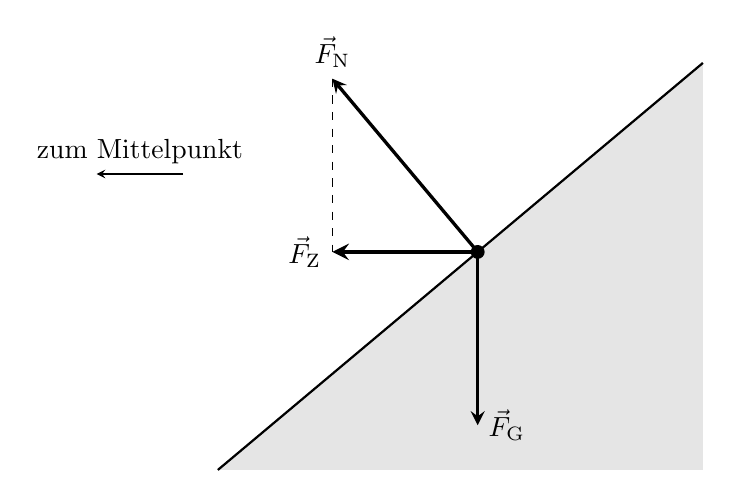
\begin{tikzpicture}[>=stealth, scale=1.1]
 \fill[gray!20] (-3,-2.517) -- (2.6,2.182) -- (2.6,-2.517) -- cycle;
 \draw[thick] (-3,-2.517) -- (2.6,2.182);
 \fill (0,0) circle (0.08);
 \draw[->, very thick] (0,0) -- (-1.678,2.0) node[above] {$\vec F_\mathrm{N}$};
 \draw[->, very thick] (0,0) -- (0,-2) node[right] {$\vec F_\mathrm{G}$};
 \draw[dashed] (-1.678,2.0) -- (-1.678,0);
 \draw[->, ultra thick] (0,0) -- (-1.678,0) node[left] {$\vec F_\mathrm{Z}$};
 \draw[->] (-3.4,0.9) -- (-4.4,0.9) node[midway, above] {zum Mittelpunkt};
\end{tikzpicture}
\end{center}
